\section{Simulation Analysis}
\label{sec:simulation}

\paragraph{}
In this section, we can find the results of the topics required in the simulation analysis. The numeric results or graphics are presented. All of the results were obtained using NGSpice. 

Taking in consideration the components that we were allowed to use during this laboratory class, we tried to find the best values for the bandpasss filter circuit to achieve the main goal of the assignment, which was to obtain a value for the central frequency around 1000 Hz, and a value for the gain in the central frequency around 40 dB. With the simulation finished, we were finally able to obtain the following results:

\begin{figure}[H]\centering
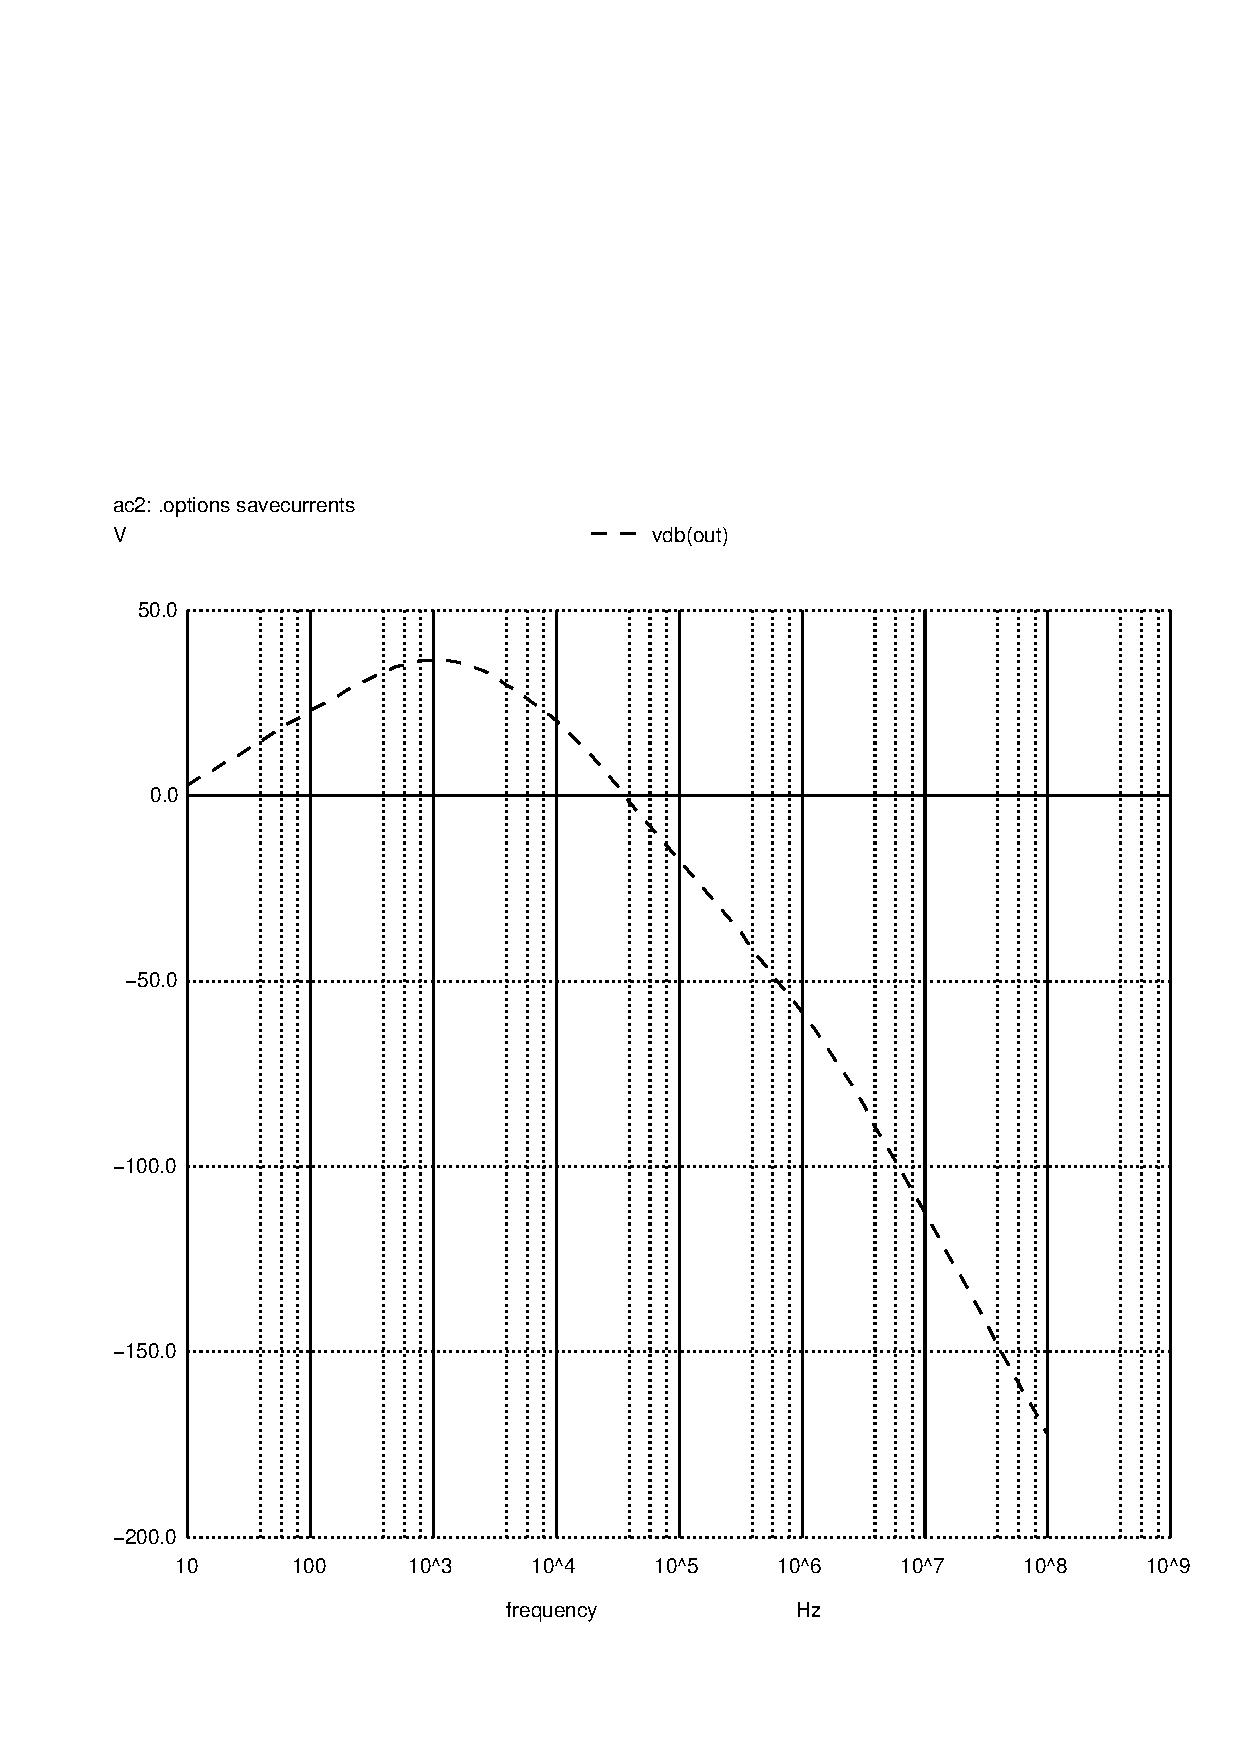
\includegraphics[width=0.7\linewidth]{gain.pdf}
\caption{Simulated frequency response - gain[dB]}
\label{fig:sim_output}
\end{figure}

\begin{figure}[H]\centering
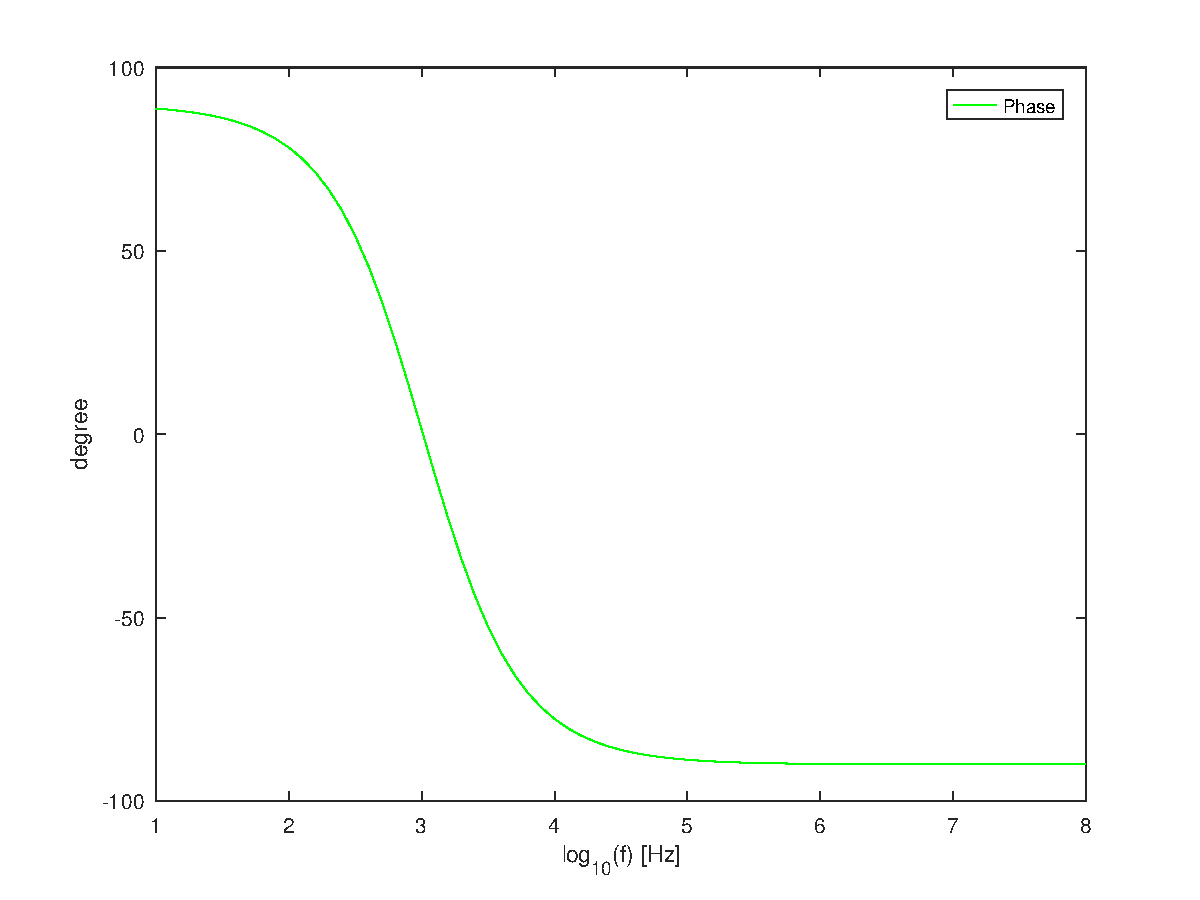
\includegraphics[width=0.7\linewidth]{phase.pdf}
\caption{Simulated frequency response - phase[deg]}
\label{fig:sim_output2}
\end{figure}

\begin{table}[H]
\centering
\begin{tabular}{|l|l|} 
\hline
\textbf{Characteristics} & \textbf{Values}  \\ \hline
Gain & 67.0836 V\\ \hline
Gain dB & 36.5323 dB\\ \hline
Gain Deviation & 3.4677 dB\\ \hline
Lower Cut Off Frequency & 406.808 Hz\\ \hline
Higher Cut Off Frequency & 2481.27 Hz\\ \hline
Central Frequency & 1004.69 Hz\\ \hline
Frequency Deviation & 4.69 Hz\\ \hline
Bandwidth & 2074.46 Hz\\ \hline
Input Impedance & 1234.29 Ohm\\ \hline
Output Impedance & 824.902 Ohm\\ \hline
\end{tabular}
\end{table}

\paragraph{}
The interpretation of the graphic allows us to see that our work was successfull. Not only we were able to obtain similar values to the required specifications for the central frequency (1004.69 Hz compared to the 1000 Hz) and for the gain at central stage (36.5323 dB compared to the 40 dB) but also taking into account that a bandpass filter circuit is a circuit that is designed to filter not only high but low frequencies (hence its name: it can filter specific frequency ranges), taking a closer look at the table, we can see that this goal was achieved.

\paragraph{}
The impedances are also very important values to obtain when trying to interpret the viability of the circuit. And that's why it is really important to calculate the input impedance and the output impedance. Analysing the values obtained through simulation, we can safely say they were quite satisfactory: we wanted a relatively high value for the input impedance (which was achieved), and a very low value for the output impedance, as we desire a high output voltage value (which was also achieved).

